\begin{center}
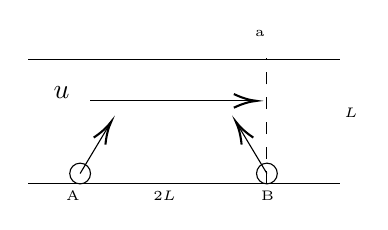
\begin{tikzpicture}[x=0.75pt,y=0.75pt,yscale=-1,xscale=1]
%uncomment if require: \path (0,300); %set diagram left start at 0, and has height of 300

%Straight Lines [id:da21927273521379798] 
\draw    (120,80) -- (270,80) ;
%Straight Lines [id:da4378923778307051] 
\draw    (120,140) -- (270,140) ;
%Shape: Circle [id:dp7352837546468081] 
\draw   (140,135) .. controls (140,132.24) and (142.24,130) .. (145,130) .. controls (147.76,130) and (150,132.24) .. (150,135) .. controls (150,137.76) and (147.76,140) .. (145,140) .. controls (142.24,140) and (140,137.76) .. (140,135) -- cycle ;
%Shape: Circle [id:dp41722119373569155] 
\draw   (230,135) .. controls (230,132.24) and (232.24,130) .. (235,130) .. controls (237.76,130) and (240,132.24) .. (240,135) .. controls (240,137.76) and (237.76,140) .. (235,140) .. controls (232.24,140) and (230,137.76) .. (230,135) -- cycle ;
%Straight Lines [id:da7158120985157417] 
\draw    (145,135) -- (158.97,111.71) ;
\draw [shift={(160,110)}, rotate = 120.96] [color={rgb, 255:red, 0; green, 0; blue, 0 }  ][line width=0.75]    (10.93,-3.29) .. controls (6.95,-1.4) and (3.31,-0.3) .. (0,0) .. controls (3.31,0.3) and (6.95,1.4) .. (10.93,3.29)   ;
%Straight Lines [id:da9687396877898515] 
\draw    (235,135) -- (221.03,111.71) ;
\draw [shift={(220,110)}, rotate = 59.04] [color={rgb, 255:red, 0; green, 0; blue, 0 }  ][line width=0.75]    (10.93,-3.29) .. controls (6.95,-1.4) and (3.31,-0.3) .. (0,0) .. controls (3.31,0.3) and (6.95,1.4) .. (10.93,3.29)   ;
%Straight Lines [id:da22872254896655053] 
\draw    (150,100) -- (228,100) ;
\draw [shift={(230,100)}, rotate = 180] [color={rgb, 255:red, 0; green, 0; blue, 0 }  ][line width=0.75]    (10.93,-3.29) .. controls (6.95,-1.4) and (3.31,-0.3) .. (0,0) .. controls (3.31,0.3) and (6.95,1.4) .. (10.93,3.29)   ;
%Straight Lines [id:da5167178486268149] 
\draw  [dash pattern={on 4.5pt off 4.5pt}]  (235,140) -- (235,79.5) ;

% Text Node
\draw (271,102) node [anchor=north west][inner sep=0.75pt]  [font=\tiny] [align=left] {$\displaystyle L$};
% Text Node
\draw (137,142) node [anchor=north west][inner sep=0.75pt]  [font=\tiny] [align=left] {A};
% Text Node
\draw (231,142) node [anchor=north west][inner sep=0.75pt]  [font=\tiny] [align=left] {B};
% Text Node
\draw (179,142) node [anchor=north west][inner sep=0.75pt]  [font=\tiny] [align=left] {$\displaystyle 2L$};
% Text Node
\draw (131,92) node [anchor=north west][inner sep=0.75pt]   [align=left] {$\displaystyle u$};
% Text Node
\draw (228,65) node [anchor=north west][inner sep=0.75pt]  [font=\tiny] [align=left] {a};


\end{tikzpicture}

\end{center}